Content similarity within a single VM image is called intra-VM similarity and across multiple
VMs is referred to as inter-VM similarity. A study of content similarity amongst 525 VM images
from a production environment~\cite{similarity}
reported 30\% blocks repeating at least twice and 12\% blocks
repeating 5 times. A study in \cite{intra-higherthan-inter} 
reported that up to 90\% of total similarity observed among VM
disk content is intra-VM, rather than inter-VM. 
The work in \cite{iodedup} 
studied the degree of content
similarity in application workloads (web, mail and file system) hosted in VMs, and reported that
there are multiple blocks having identical content within each application workload.

A VM's virtual disk is present on the host's storage, which may be a local disk 
or a network-attached remote disk. 
Disk access times are in the order of a few 
milliseconds~\cite{google, data-domain}, whereas cache
access timings are orders of magnitudes lower~\cite{pagecache, satori}. 
Hence, improving caching effectiveness can
help improve storage access performance and overall application performance. However, due to
content similarity across blocks, host cache effectiveness is limited by two factors: (i) duplicate
I/O problem\textemdash{}multiple blocks containing same content being fetched from disk, 
and (ii) duplicate content problem\textemdash{}multiple blocks in cache have same content. 
Both problems can be
addressed by maintaining content similarity metadata by actively tracking insertion and eviction
of blocks in page cache, however this would require invasive changes in the host kernel.
We develop a read I/O redirection technique positioned within the VM's virtual block device,
such that both problems are addressed. If a block of content is present in the host's page-cache,
it need not get fetched from disk. This, in turn, ensures that multiple blocks with same content
are (almost) never stored into the host's page-cache, i.e., a content-deduplicated page-cache is
achieved. Thus, we reduce disk I/O without actively tracking page-cache state, as well as without
maintaining any explicit content cache. The \textbf{contributions} of this work are,
\begin{enumerate}
	\singlespacing
\item Simulation-based analysis of existing system \cite{iodedup} to show that it is sub-optimal.
\item Design and implementation of the DRIVE system that tackles both the duplicate content
and duplicate I/O problems,
\item Trace-based evaluation of DRIVE with prototype implementation in a custom simulator.
\end{enumerate}

\begin{table}
%\vspace{0.1in}
\caption{Summary statistics of traces used for evaluation}
\label{tab:stat-summary}
\centering
%\noindent\makebox[\textwidth]{% 
\begin{tabular}{|l|c|c|c|c|c|c|c|} \hline
	\textbf{Trace} & \textbf{Num of} & \textbf{Num of} & \textbf{Max} & \textbf{Max} & \textbf{\%blks} & \textbf{\%content} & \textbf{Write} \\
	 \textbf{Name} & \textbf{read} & \textbf{write} & \textbf{share} & \textbf{occur} & \textbf{having} & \textbf{occuring} & \textbf{intensivity} \\
			   \textbf{} & \textbf{requests} & \textbf{requests} & \textbf{factor} & \textbf{factor} & \textbf{2 copies} & \textbf{twice} & \textbf{factor}  \\ \hline
	\textit{homes} & 4,052,176 & 17,110,222 & 5904 & 5905 & 5 & 10 & 4.2 \\ \hline
	 \textit{mail} & 2,375,409 & 18,007,471 & 57015 & 57015 & 5 & 6 & 7.6 \\ \hline
	\textit{webvm} & 3,116,456 & 11,177,702 & 124 & 125 & 35 & 45 & 3.6 \\ \hline
\end{tabular}
%}
%\vspace{-0.3in}
\end{table}

\begin{figure}
	\RawFloats
	\begin{minipage}{0.45\textwidth}
	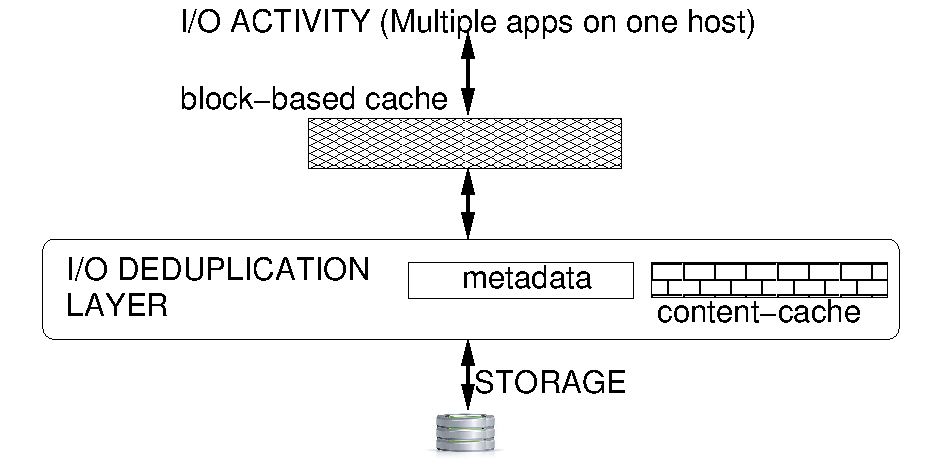
\includegraphics[scale=0.55]{confided-figures/main/sys-arch-iodedup-host.pdf}
	\vspace{-0.25in}
	\caption{System Architecture of IODEDUP}
	\label{fig:iodedup-arch}
	%\vspace{-0.2in}
	\end{minipage}
	\hfill
	\begin{minipage}{0.47\textwidth}
	    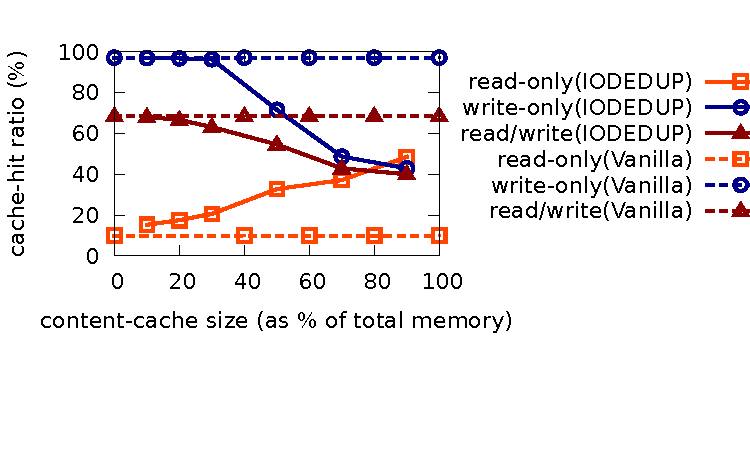
\includegraphics[scale=0.60]{confided-figures/sweetspot-512MB/sweetspot-512MB.pdf}
			\vspace{-0.5in}
			\caption{Hit ratios in IODEDUP upon \textit{webvm}; total cache size is 512 MB.}
			\vspace{-0.05in}
			%, and content-cache size as the specified \% of the total.}
			\label{fig:sweetspot-512MB}
		\end{minipage}
\end{figure}
\vspace{-0.2in}

%\vspace{-0.2in}
\subsection{Analysis of existing I/O deduplication technique: IODEDUP}
Harnessing content similarity to avoid duplicate disk I/O requests is called I/O deduplication.
The work in \cite{iodedup} 
builds metadata regarding block content similarity, and maintains a content-
cache\textemdash{}retains a single copy of each content. Fig.~\ref{fig:iodedup-arch} 
shows I/O Deduplication (henceforth IODEDUP) system architecture. 
When read requests encounter a block-cache miss, they are 
intercepted by IODEDUP system and serviced from content-cache, if possible\textemdash{}thus avoiding 
duplicate content fetches from disk. However, since only a fraction of total space can be reserved
as content-cache, the \underline{duplicate content problem persists}. 
Secondly, since the content-cache
partakes from total memory space available, 
\underline{optimally sizing the content-cache is essential}
because content-cache benefits may be application or request-mix specific.

\vspace{-0.2in}
\paragraph{Simulation setup:} We built a custom simulator, \texttt{SimReplay}, 
with prototype implementations
of Vanilla and IODEDUP systems. In Vanilla system, a read request's block number is first
looked up into block-cache. If not found in cache, the block is fetched
from disk. In IODEDUP system, the disk fetch path due to block-cache miss is intercepted 
and metadata is used to lookup the block in content-cache. A content-cache hit averts
the disk fetch, however, a miss necessitates disk fetch and metadata update. For exploration of
IODEDUP system's effectiveness, we chose six content-cache size settings as 10\%, 20\%, 30\%,
50\%, 70\% and 90\% of the total memory size, and remaining as the block-cache size.

\vspace{-0.2in}
\paragraph{Traces for simulation:} We borrow traces provided via \cite{iodedup} 
which are over 21 days from three
production systems: (i) webvm--from virtualized web-servers hosting webmail proxy and course
management system, (ii) mail--email server traces, and (iii) homes--file server traces. 
Table \ref{tab:stat-summary}
presents a summary of the traces. %, shows that webvm workload is likely to benefit most from
%deduplication techniques, due to higher percentage of content sharing and occurrence.

\vspace{-0.2in}
\paragraph{Analysis results:} Fig.~\ref{fig:sweetspot-512MB} 
shows cache-hit ratios for webvm trace for read-only, write-only and
read-write replays. IODEDUP has different optimal content-cache sizes for different 
cases\textemdash{}90\% for read-only, 10\% for write-only, and 10\% for read/write. 
Further, for read-write trace, performance of IODEDUP worsens compared to Vanilla, 
as content-cache size increases. Hence,
we consider 10\% as optimal content-cache size for further evaluation.

\begin{figure}
	\RawFloats
	\begin{minipage}{0.4\textwidth}
    \centering
    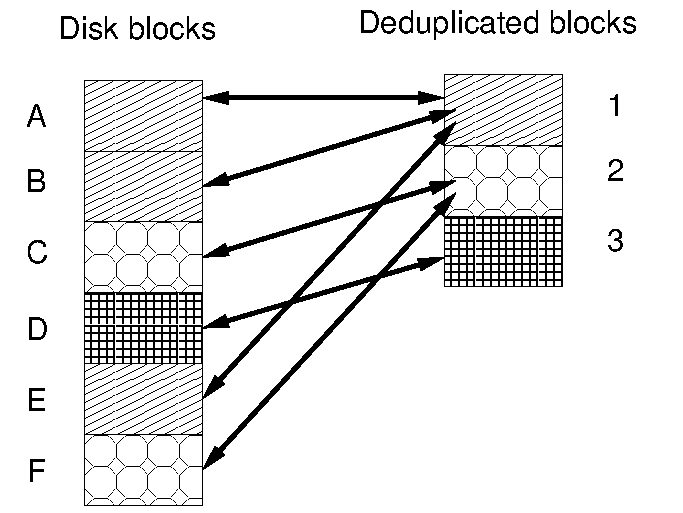
\includegraphics[scale=0.5]{confided-figures/main/deduped-block.pdf}
%    \vspace{-0.15in}
%    \caption{Semantics of metadata store in DRIVE system: \textit{each block points to a unique deduplicated block, and each deduplicated block reverse maps to multiple actual blocks}}
	\caption{Metadata store semantics: \textit{each block points to a unique deduplicated block, and each deduplicated block reverse maps to multiple actual blocks}}
    \label{fig:deduped-block}
%    \vspace{-0.2in}
	\end{minipage}
	\hfill
	\begin{minipage}{0.55\textwidth}
    \centering
    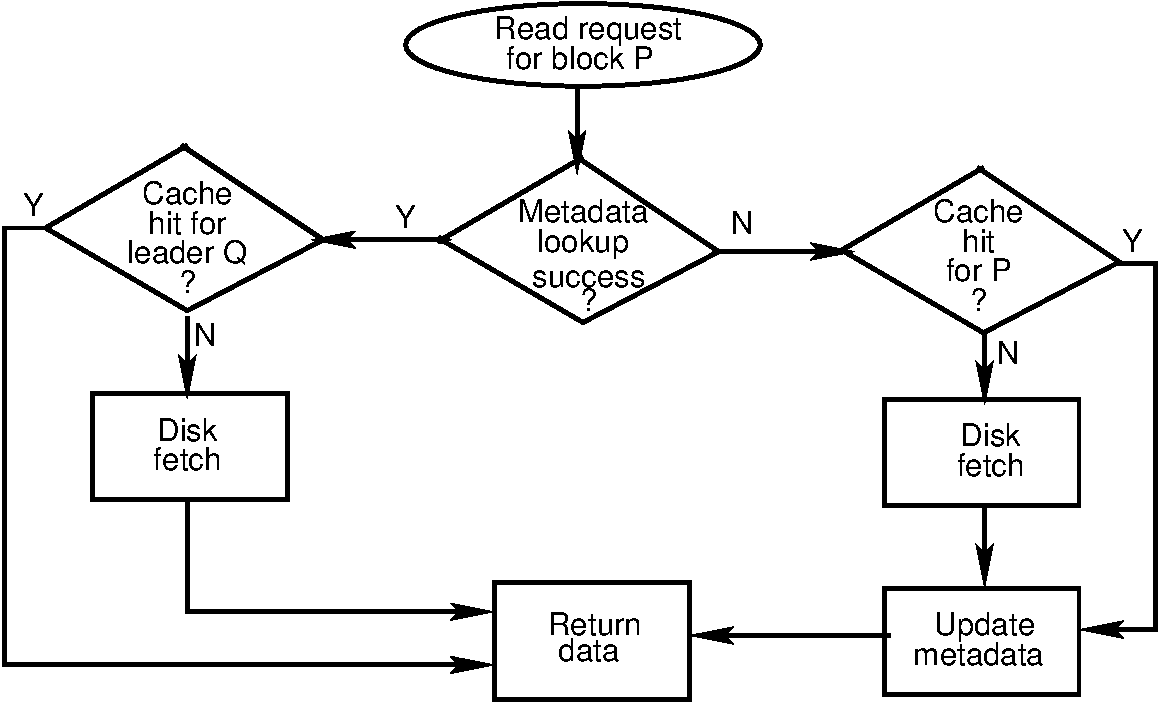
\includegraphics[scale=0.5]{confided-figures/main/dedup-working-readflowcomp.pdf}
    \caption{Flow path(s) for read in DRIVE: \textit{P is requested block, Q is corresponding ``leader'' block.}}
    \label{fig:confided-working(b)}
%     \vspace{-0.25in}
	\end{minipage}
\end{figure}
\vspace{-0.2in}


\subsection{DRIVE system requirements and design}
We build an I/O redirection system positioned above the block-cache which uses implicit caching
hints to perform the redirection.
%\vspace{-0.2in}
%\paragraph{System requirements.} 
The \textbf{system requirements} of an efficient I/O reduction system:
\begin{enumerate}
	\singlespacing
	\small
\item Fingerprinting mechanism to identify content similarity across different blocks.
%\item Data-structures to store metadata for similar blocks.
\item Maintaining implicit caching hints within metadata to aid future I/O redirection.
\item Interception of block read request path for metadata lookup and I/O redirection, if present.
\item Interception of block read return path for metdata update, if not previously present.
\item Interception of block write request path for metadata invalidation.
\end{enumerate}

\vspace{-0.2in}
\paragraph{System Design.} 
The DRIVE system has three main components: (i) \textit{Metadata maintenance},
(ii) \textit{Maintaining implicit hints regarding host-cache state}, 
(iii) \textit{Hint-based read I/O redirection}.

\textbf{(i)~Metadata maintenance}: 
%Metadata is updated for every new block of content , encountered
%in two ways: (i) every block of data written to cache, %for later flushing to disk, 
%(ii) every read
%request for an as yet unseen block fetched from disk. 
For read requests,
we compare content fingerprints to determine whether it is ``new'' or ``duplicate'', and
update metadata accordingly. For write requests, we invalidate existing mappings for those
blocks, so that stale metadata is not used for the next read request redirection.
The semantics of metadata store is as illustrated 
in Fig.~\ref{fig:deduped-block}.

\textbf{(ii)~Maintaining hints regarding host-cache state}: 
To avoid invasive tracking of host-cache (i.e., by trapping and intercepting each 
insertion and eviction within cache), we use \textit{implicit hints}
for redirection instead. When a read request is serviced, the corresponding physical block is in
host-cache, and if found to be identical to any previously requested block, we record the current
block ID as ``leader'', for that content. The recording as leader is done to aid redirection of future
I/O requests that request the same content, and is a hint regarding the state of host-cache.
%, and do not
%guarantee a cache-hit. However, hints offer a good chance of encountering a cache-hit to fetch
%the same content, without explicitly tracking host-cache.

\begin{figure}
    \RawFloats
    \begin{minipage}{0.45\textwidth}
    \centering
    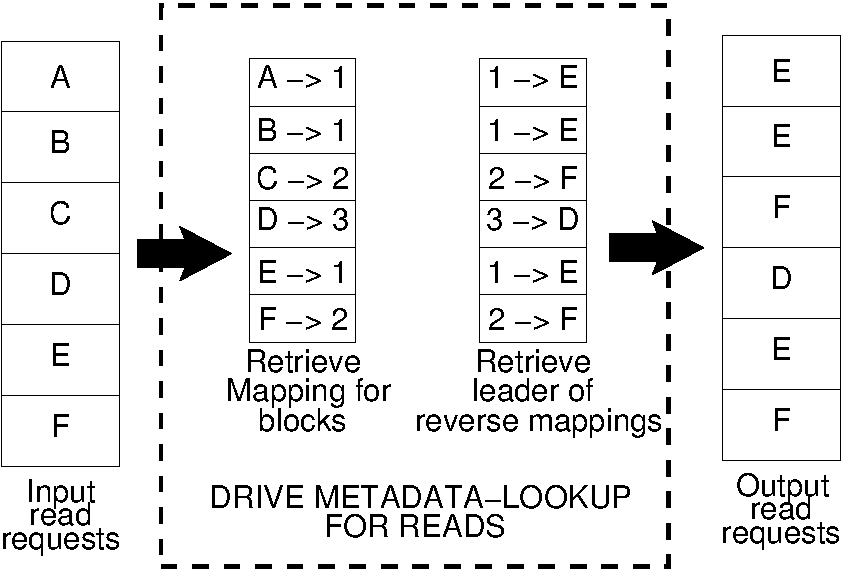
\includegraphics[scale=0.5]{confided-figures/main/dedup-working-reads.pdf}
%    \vspace{-0.125in}
    \caption{Read request redirection in DRIVE}
    \label{fig:confided-working(a)}
%    \vspace{-0.15in}
	\end{minipage}
	~~~~~
    \begin{minipage}{0.55\textwidth}
    \centering
	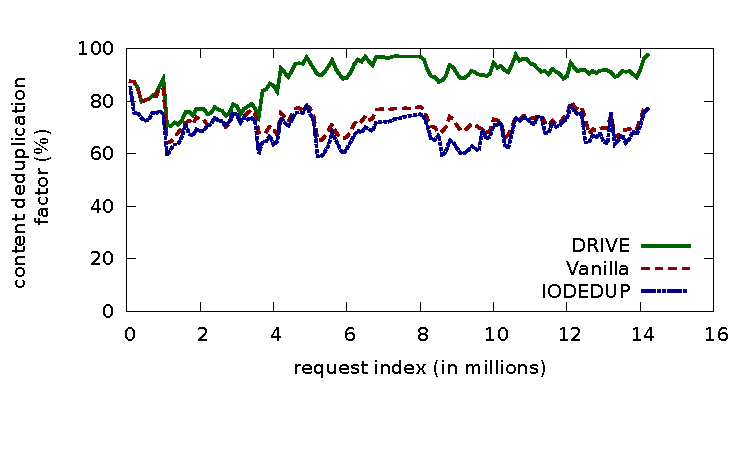
\includegraphics[scale=0.8]{confided-figures/contentdedup-factor/contentdedupfactor.pdf}
	\vspace{-0.6in}
	\caption{Host cache effectiveness upon \textit{webvm} trace.}
	\label{fig:contentdedup-factor-timeseries}
%    \vspace{-0.2in}
	\end{minipage}
\end{figure}

\textbf{(iii)~Read I/O redirection using implicit hints}: 
Before a read request hits the host-cache, the DRIVE
system intercepts it and looks up metadata to check for a recorded leader. If present, original
block ID in request is replaced with the leader block ID. Fig.~\ref{fig:confided-working(b)} 
depicts the multiple flows in
the read path, wherein an incoming request for block P is looked up in metadata store and if
successful, redirected to block Q.

\underline{Overall operation}: Fig.~\ref{fig:confided-working(a)} 
illustrates via an example. Suppose blocks A, B and E have identical
content (mapped to deduplicated ID 1) and E is appointed their leader since it was fetched the
latest. Whenever next, read requests for A, B or E are received, request is redirected to read
block E. Note that, blocks A, B and C will be in cache the first time they are fetched but once
they get evicted, they will never enter cache again, unless writes are done to them. This implies
that the cache is operated in an almost fully content-deduplicated fashion, hence improving its
effectiveness in reducing the number of disk reads.

%\vspace{-0.2in}
%%\paragraph{System implementation.} Fig.~\ref{fig:metadata-structure} 
%shows summary of metadata store 
%implementation\footnote{The CPU and memory overhead analysis is present in the thesis}. It con
%sists of an array containing entries for every block, a hash-table containing entries for every
%deduplicated block, and an array of pointers indexed by deduplicated block ID, pointing to the
%corresponding entry in hash-table. Each hash-table entry corresponds to one deduplicated block,
%has a list of reverse mapped block IDs, as well as content fingerprint. The fingerprint technique,
%used for duplicate content identification, can be any collision-resistant hash function. For leader
%identification, the list of reverse mappings is a Last-in-First-Out (LIFO) list. If the leader block
%content changes due to a write request, it is removed from the list of reverse mappings and the
%next most recently fetched block ID becomes new leader.

%\begin{figure}[t]
%%   \centering
%    \subfloat[Cache-hit performance]{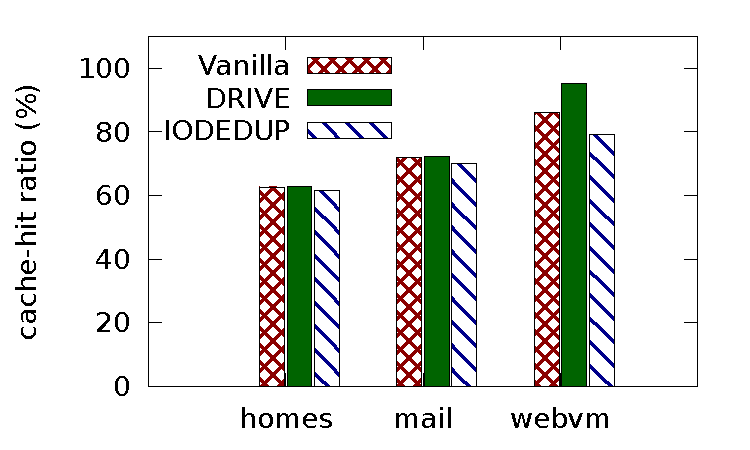
\includegraphics[scale=0.55]{confided-figures/cache-hit-rate/reads-writes/eval-reads-n-writes.pdf}} \hfill
%    \subfloat[Disk read reduction]{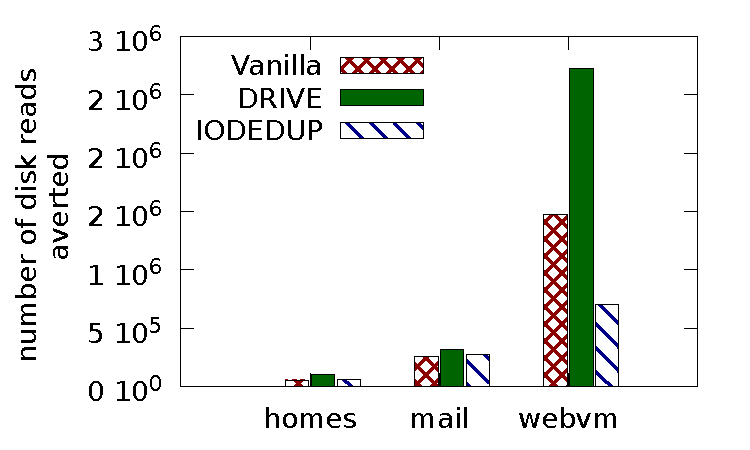
\includegraphics[scale=0.55]{confided-figures/disk-fetches-averted/reads-writes/readsaverted-reads-n-writes.pdf}}
%    \caption{Comparison based on \textit{measured metrics} for read/write traces}
%    \label{fig:eval-read-write-perf-a}
%	\vspace{-0.1in}
%\end{figure}

%\begin{figure}
%    \RawFloats
%    \begin{minipage}{0.4\textwidth}
%    \centering
%    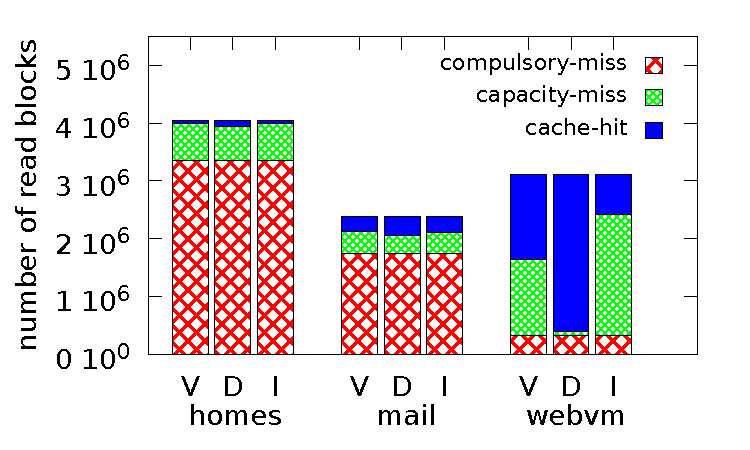
\includegraphics[scale=0.49]{confided-figures/read-response-distrib/reads-writes/read-response-distrib-reads-n-writes.pdf}
%    \caption{Classification of read responses in Vanilla Vs IODEDUP Vs DRIVE for \textit{homes}, \textit{mail} and \textit{webvm}.}
%    \label{fig:eval-read-write-perf-c}
%	\end{minipage}
%	\hfill
%    \begin{minipage}{0.59\textwidth}
%	\centering
%	%\vspace{-0.1in}
%	\end{minipage}
%\end{figure}
%\vspace{-0.2in}

\subsection{Summary of experimental evaluation}
For evaluation, we extend our simulator, and replay same traces as before. 
%Every record in the
%trace file contains:- (i) block number to be read or written, and (ii) MD5 hash of content. 
For every trace replay, measures like cache hits, cache misses, and disk fetches are recorded.
We performed evaluation for individual (single-VM) 
workloads, as well as simultaneous (multi-VM) workloads. 
Here, we present a summary list of main results.

\begin{enumerate}
	\item Our evaluation shows that with webvm workload,
		DRIVE has \underline{higher cache-hit ratios} than both 
		Vanilla and IODEDUP systems, 10\% and 20\% better, respectively.
		Moreover, DRIVE has higher number of ``disk reads reduced'', with nearly
		85\% improvement over Vanilla, and a 2.8$\times$ improvement over IODEDUP.
	\item A \underline{classification of read request responses} into compulsory misses, capacity misses
		and cache hits, for each trace, showed that \textit{webvm} trace contained a
		lot of capacity misses in the Vanilla system, and DRIVE succeeds in reducing 
		them to 5\% of the Vanilla system.
	\item We define \underline{content deduplication factor} as the ratio of
number of unique content blocks to total number of blocks in cache. Thus, higher the content
deduplication factor, better is cache efficiency. Fig.~\ref{fig:contentdedup-factor-timeseries} 
shows the variation in content deduplication factor, as each request of the webvm trace is replayed. We see that DRIVE system achieves
significantly higher content deduplication than both Vanilla and IODEDUP\textemdash{}a content 
deduplication factor of up to 97\%.
	\item To perform \underline{evaluation of multi-VM workloads} executed on a 
		virtualized host, we aggregated the \textit{homes} and \textit{webvm} 
		traces in timestamp order, and replayed it.
The metrics tabulated in Table~\ref{tab:aggregate-hw} 
show that although the cache-hit ratios are comparable in all
three schemes, DRIVE system averts 18\% disk reads as compared to 1.6\% of Vanilla and 4.3\%
of IODEDUP. Fig.~\ref{fig:aggregate-hw-time-series} 
plots the read response throughput per hour, assuming continuous replay
of requests. We can see that DRIVE produces more number of responses per hour in the 4th,
5th, 6th hours and so on, hence resulting in earlier completion than Vanilla or IODEDUP.
\end{enumerate}

%content deduplication of page cache can not be achieved because of compulsory misses incurred
%during cache-warmup, as well as cache dirtying by write requests. However, 
%DRIVE attains a high content deduplication factor of up to 97\%.

\begin{figure}
\begin{floatrow}
\ffigbox{%
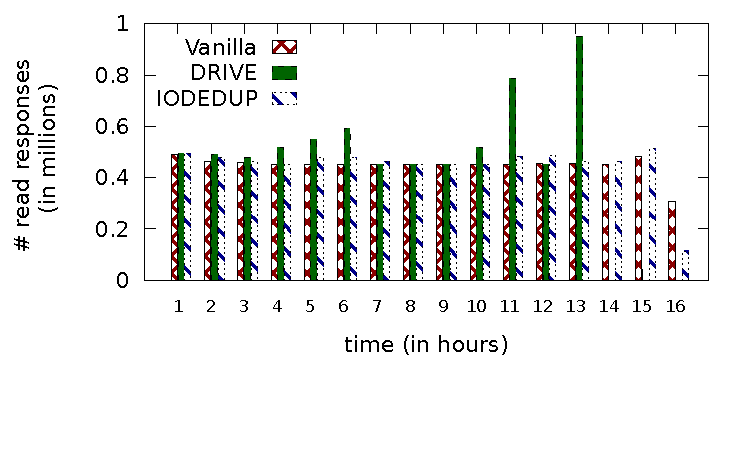
\includegraphics[scale=0.7]{confided-figures/aggregate-hw-replay/reads-writes/timeseriesperf-hour.pdf}
}{%
\caption{Read throughput for aggregate trace}
\vspace{-0.55in}
\label{fig:aggregate-hw-time-series}
}
~~~
\vspace{-0.1in}
\capbtabbox{%
\begin{tabular}{|c|c|c|} \hline
\textbf{Scheme} & \textbf{Hit} & \textbf{Reads} \\
\textbf{} & \textbf{rate(\%)} & \textbf{saved(\%)} \\ \hline
%\textbf{} & \textbf{} & \textbf{} & \textbf{latency} \\ \hline
Vanilla & 61.2 & 1.6 \\ \hline
DRIVE & 67.6 & 18.5 \\ \hline
IODEDUP & 62.4 & 4.3 \\ \hline
\end{tabular}
}{%
	\caption{Aggregate replay performance}
	\label{tab:aggregate-hw}
}
\end{floatrow}
\end{figure}

\vspace{-0.05in}
\subsection{Conclusions}
In this section,
we considered the problem of improving disk access performance by improving host
cache efficiency. Typically, caches are referenced by block number, and can not recognize con-
tent similarity across multiple blocks. 
%Hence, the system ends up storing multiple copies of same content into cache. 
Elimination of duplicate read I/O requests is referred to as I/O Deduplication.
Existing work (IODEDUP) uses a split-cache approach~\cite{iodedup}, 
with a part of block-cache reserved as a content-cache. 
We demonstrated that a split-cache approach is sub-optimal, and presented
the DRIVE system which performs I/O redirection to implicitly manipulate the whole underlying
cache as a content-deduplicated cache. Only the VM's own disk access history is introspected
to obtain implicit hints regarding host cache state, to be used for read I/O redirection.

We performed comparative trace-based evaluation in a custom simulator. The evaluations
showed that, the DRIVE system achieves a high content deduplication factor of up to 97\%. This
is the key reason for better performance, with up to 20\% higher cache-hit ratios, and up to 85\%
higher number of disk reads reduced than the Vanilla system.


%\subsection{Discussion and future work}
%\paragraph{Further evaluation.} Based on an extensive literature survey of 100+ publications and 350+
%datasets, we concluded that there are no realistic benchmarking tools or trace generation frame-
%works for evaluation of I/O deduplication techniques. Thus, we need to either collect multiple
%production workload traces, or create frameworks that can synthesize realistic I/O traces having
%content representation, for further research in this area.
%\paragraph{Applicability to other storage systems.} The IODEDUP system uses ARC policy to boost
%up its content-cache hit ratio by 3-4X~\cite{}. 
%DRIVE performance could also get a boost if the
%host-cache policy is changed to ARC. Although this is unlikely in a standard Linux host, ARC
%caches are present in IBM's DS6000/DS8000 storage controllers, so adoption of DRIVE may
%help increase their cache performance.



